\chapter{Analisi dei dati di ALICE} \label{Analisi}


\section{I Dati Iniziali}

I dati che si vogliono analizzare in questa tesi sono relativi a collisioni di due fasci di protoni ad un'energia nel centro di massa di 5 TeV e sono stati raccolti da ALICE nel 2017. 
\\Dall'insieme delle particelle prodotte nella collisione dei due fasci si vogliono identificare i mesoni $D^{*+}$, ricostruendo il decadimento $D^{*+} \rightarrow D^0(\rightarrow \pi^+ k^-) \pi^+ $. L'estrazione del segnale \`e stata fatta in diversi intervalli di impulso trasverso $p_T$ delle candidate $D^{*+}$: [1,2], [2,3], [3,4], [4,5], [5,6], [6,8], [8,12] misurati in GeV/c. Tutte le possibili combinazioni delle tracce di due $\pi^+$ e un $K^-$ sono state pre-selezionate applicando delle selezioni minime sulle variabili discriminatorie, di cui si \`e gi\`a parlato nella sezione \ref{mesoneD}, che vengono usate per ridurre il fondo combinatoriale.
La distribuzione di massa invariante iniziale per le candidate $D^{*+}$, cioè prima dell'applicazione del BDT, è visibile in figura \ref{fig:grafmassDstar1} per l'intervallo di $p_T$ [3,4] GeV/c.

    \begin{figure}[htbp]
        \centering
        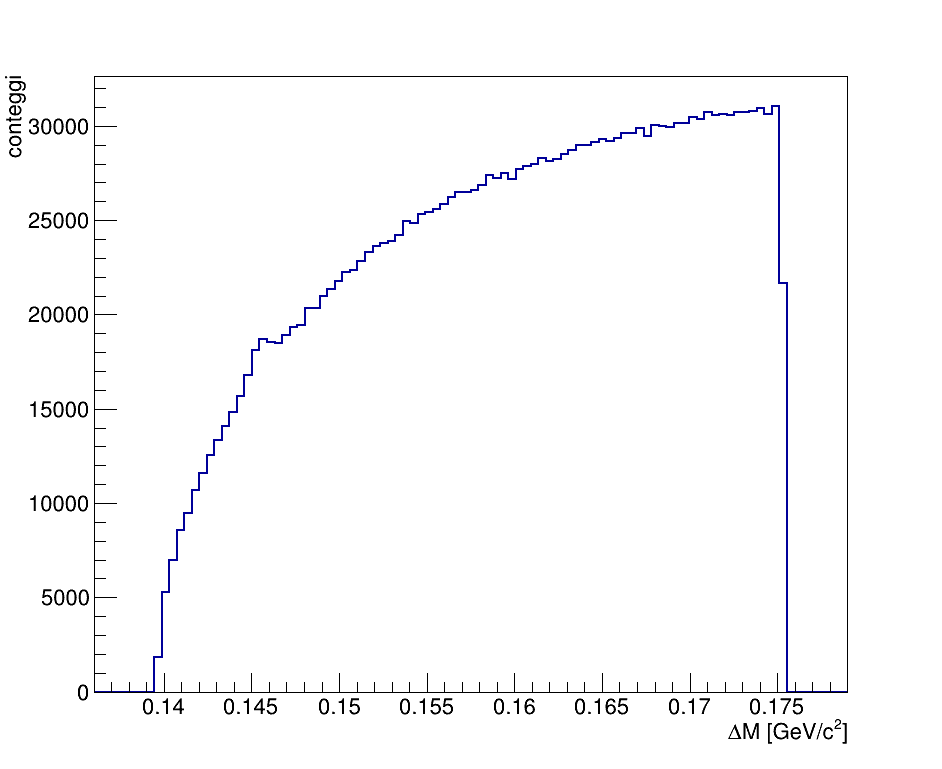
\includegraphics[width=0.7\linewidth]{AnalisiDati/diffDstarD0_3to4.png}
        \caption{Distribuzione della differenza di massa invariante tra la $D^{*+}$ e la $D^0$, $\Delta M = M(\pi^+,\pi^+,K^-) - M(\pi^+,K^-)$, per l'intervallo di $p_T$ [3,4] GeV/c prima dell'applicazione del BDT.}
        \label{fig:grafmassDstar1}
    \end{figure}
    
Nel grafico \ref{fig:grafmassDstar1} non si vede nessun picco in corrispondenza di $\Delta M = 0.145$ GeV/$c^2$. Questo accade perché il numero delle candidate $D^{*+}$ ricostruite è molto minore rispetto al fondo combinatoriale.
    \begin{figure}[htbp]
        \centering
        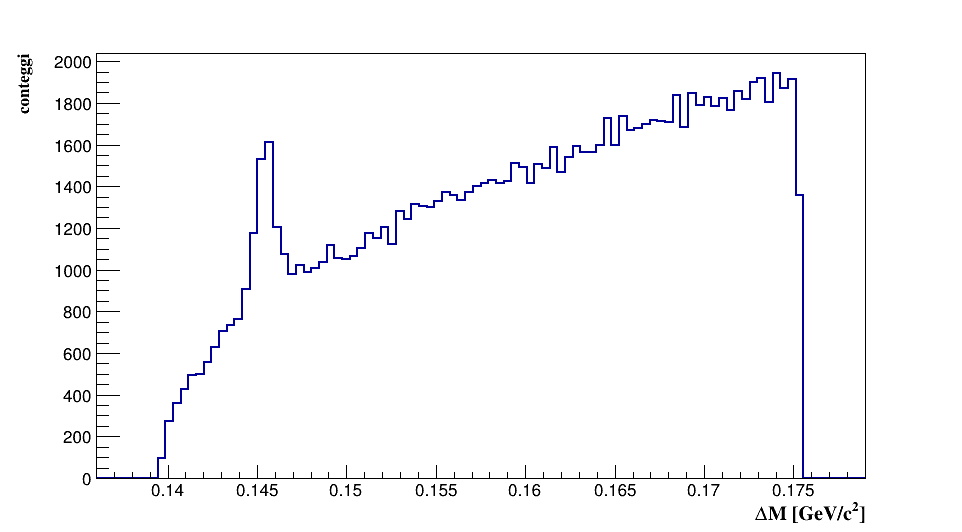
\includegraphics[width=0.7\linewidth]{AnalisiDati/dati_6_8.png}
        \caption{Distribuzione della differenza di massa invariante tra la $D^{*+}$ e la $D^0$, $\Delta M = M(\pi^+,\pi^+,K^-) - M(\pi^+,K^-)$, per l'intervallo di $p_T$ [6,8] GeV/c prima dell'applicazione del BDT}
        \label{fig:grafmassDstar2}
    \end{figure}

Al contrario, considerando un intervallo di $p_T$ pi\`u alto, [6,8] GeV/c si osserva che nella distribuzione di massa inavariante \`e gi\`a visibile il picco delle candidate $D^{*+}$, come riportato in figura \ref{fig:grafmassDstar2}. Infatti, in una collisione protone-protone vengono prodotti pi\`u $\pi^+$ e $K^-$ con basso $p_T$ che con alto $p_T$, determinando un fondo combinatoriale maggiore quando si considerano le candidate $D^{*+}$ a basso $p_T$. Dal confronto tra la figura \ref{fig:grafmassDstar1} e \ref{fig:grafmassDstar2}, \`e subito evidente che l'utilizzo di un'analisi multivariata sia pi\`u utile per candidate a basso $p_T$ che ad alto $p_T$, dove l'utilizzo di poche selezioni sulle variabili topologiche permette comunque l'identificazione del mesone $D^{*+}$.

\section{Applicazione del BDT} \label{applicazione}
Dopo aver proceduto al training e al test del BDT, l'algoritmo \`e stato applicato ai dati per separare segnale e fondo.
\\In figura \ref{fig:diffDstarD0_3_4_BDT} è riportata la distribuzione in massa invariante delle candidate $D^{*+}$ selezionate con il metodo BDT. Si vede il picco del segnale evidente attorno al valore della $ \Delta M = M(\pi^+,\pi^+,K^-) - M(\pi^+,K^-) \ \simeq \ 0.145$ GeV/c, sovrapposto ad un fondo combinatoriale residuo.

 \begin{figure}[htbp] 
        \centering
        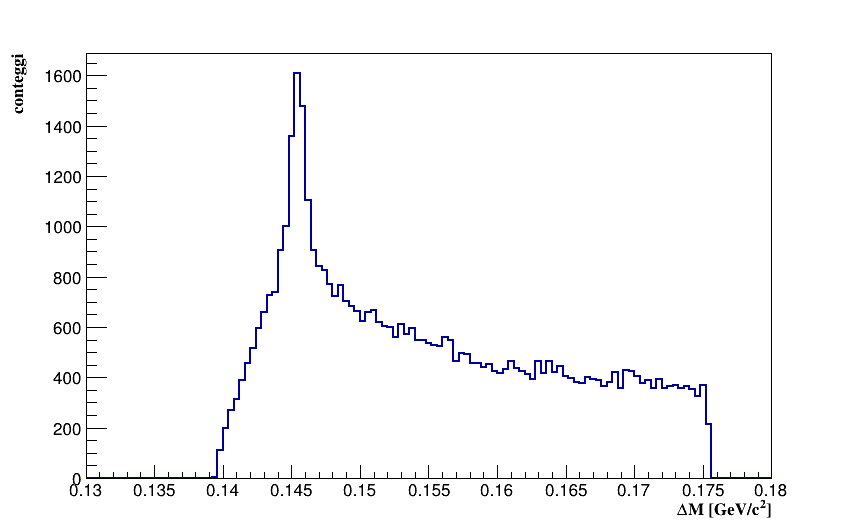
\includegraphics[width=0.7\linewidth]{AnalisiDati/diffDstarD0_3_4BDT.png}
        \caption{Distribuzione di massa invariante $\Delta M = M(\pi^+,\pi^+,K^-) - M(\pi^+,K^-)$, per l'intervallo di $p_T$ [3,4] GeV/c dopo l'applicazione del BDT}
        \label{fig:diffDstarD0_3_4_BDT}
    \end{figure}
 
Per l'intervallo di $p_T$ [1-2] GeV/c i dati della distribuzione di massa invariante delle candidate $D^{*+}$ selezionate con il metodo BDT non permettono di individuare il picco di segnale nella distribuzione di massa invariante. Per questo motivo non \`e stato possibile procedere con l'analisi per $p_T < 2$ GeV/c e perciò i risultati seguenti vengono mostrati solo per $p_T > 2$ GeV/c.   

Per determinare il numero di candidate $D^{*+}$ selezionate si è proceduto con un fit della distribuzione di massa invariante. 
Il picco del segnale é descritto da una funzione Gaussiana nell'intervallo [0.144,0.147], che corrisponde a circa 3~$\sigma$.
Per il fondo \`e stata considerata inizialmente una funzione a soglia $f_1$, tradizionalmente usata nell'analisi standard di ALICE per descrivere il fondo combinatoriale, che ha come limite inferiore la massa del $\pi^+$:
\begin{equation}
        f_1  = \ a \sqrt{x-0.13957} e^{- (x - 0.13957) }
    \end{equation}
dove la massa del $\pi^+$ vale $m_{\pi^+} = 0.13957$ GeV/$c^2$, $a$ \`e un parametro libero e la variabile $x$ corrisponde a $\Delta M$. L'intervallo considerato per la funzione $f_1$ [0.1395,0.155] \`e limitato a sinistra dal valore di soglia della massa del $\pi^+$. 
    
Per descrivere meglio il fondo nell'intervallo [0.1435,0.150] \`e stata aggiunta una funzione polinomiale di secondo grado:     
    \begin{equation}
        f_2 = \ b x^2 + c x + d
    \end{equation}
dove $b, \ c$ e $d$ sono dei parametri liberi e $x$ corrisponde a $\Delta M$. Quindi il fit del fondo combinatoriale \`e stato fatto utilizzando la funzione $f = f_1 + f_2$.

In figura \ref{fig:fit_3_4_p} si mostra il fit della funzione Gaussiana, della funzione $f$ per il fondo e la somma delle due (funzione $totale$) per l'intervallo di $p_T$ [3,4] GeV/c.
    \begin{figure}[htpb] 
        \centering
        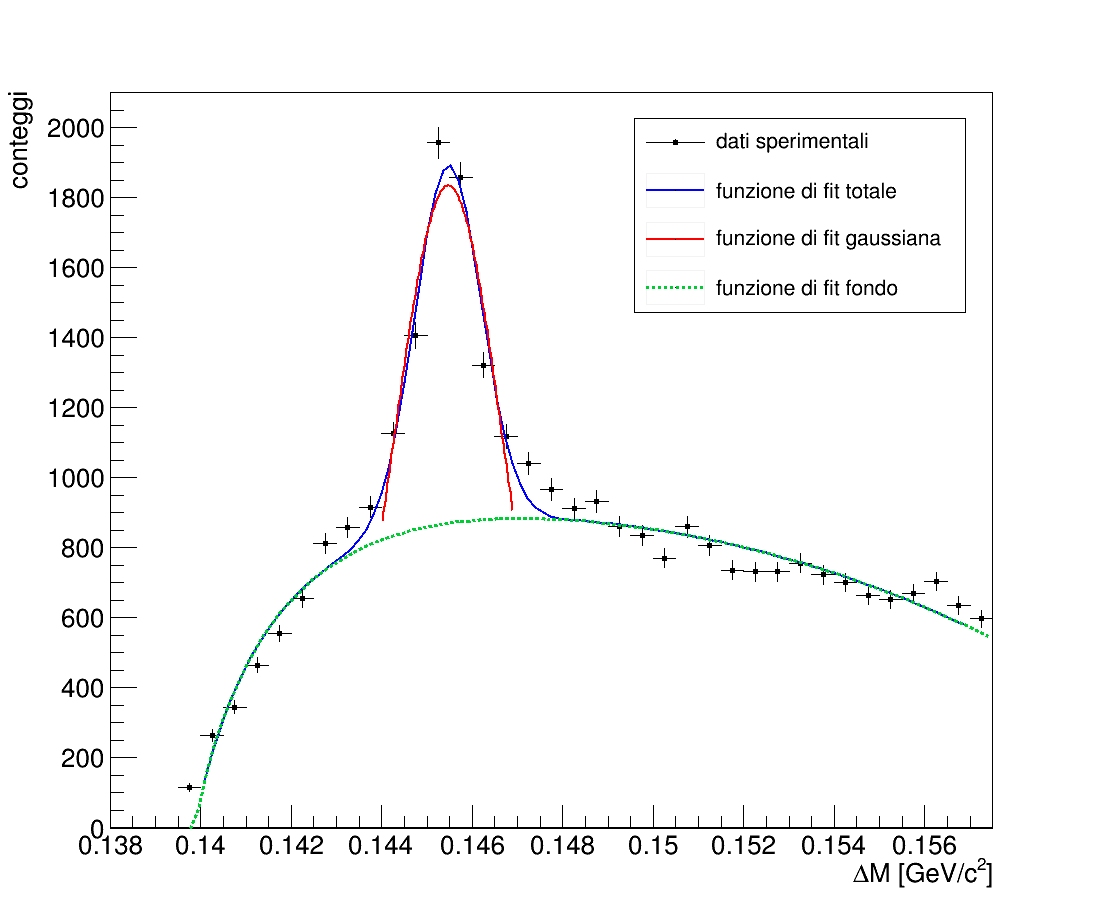
\includegraphics[width=0.8\linewidth]{AnalisiDati/fit_3_4.png}
        \caption{Distribuzione di massa invariante $\Delta M = M(\pi^+,\pi^+,K^-) - M(\pi^+,K^-)$, per l'intervallo di $p_T$ [3,4] GeV/c. Sono riportate in rosso la funzione di fit Gaussiana, in verde la funzione di fit $f$ e in blu la somma delle due funzioni (funzione $totale$). }
        \label{fig:fit_3_4_p}
    \end{figure}

Calcolando il $\chi^2$ e il numero di gradi di libert\`a ($NDL$) del fit della funzione $totale$ si \`e potuto valutare che per tutti gli intervalli di $p_T$ considerati vale $\frac{\chi^2}{NDL} < 2$. Inoltre, i risultati del fit mostrano che il picco di segnale \`e centrato nel valore $0.1455$ GeV/c, compatibile con il valore atteso. 

Nei grafici in figura \ref{fig:fit} si riportano le distribuzione di massa invariante $\Delta M$ dei dati sperimentali dopo l'applicazione del BDT con i relativi fit della funzione $totale$ per gli intervalli di $p_T$ considerati: [2,3],[3,4],[4,5],[5,6],[6,8] e [8,12].


\begin{figure}[h]      \centering
       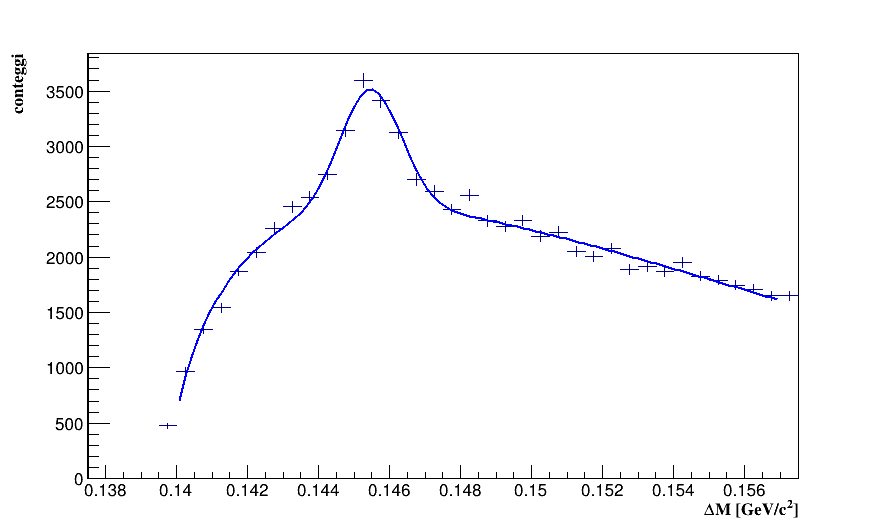
\includegraphics[width=0.48\textwidth]{AnalisiDati/pt_2_3_pol2.png}
        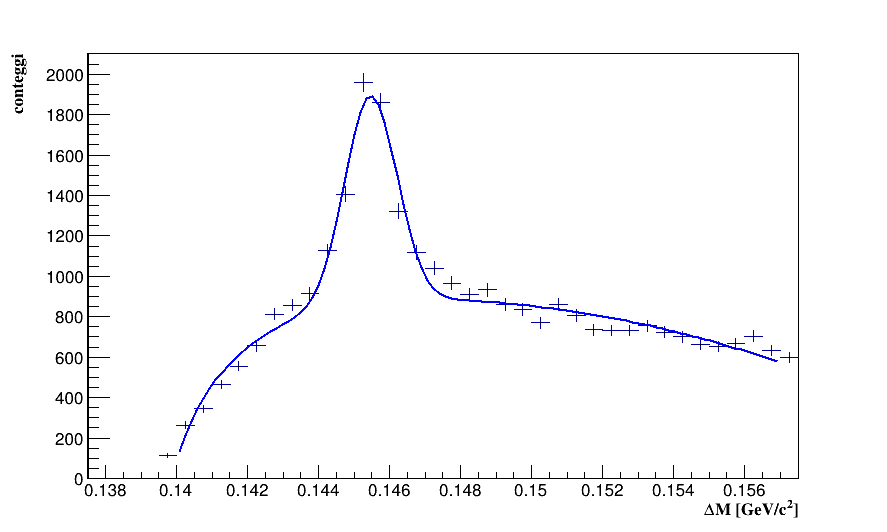
\includegraphics[width=0.48\textwidth]{AnalisiDati/pt_3_4_pol2.png}
        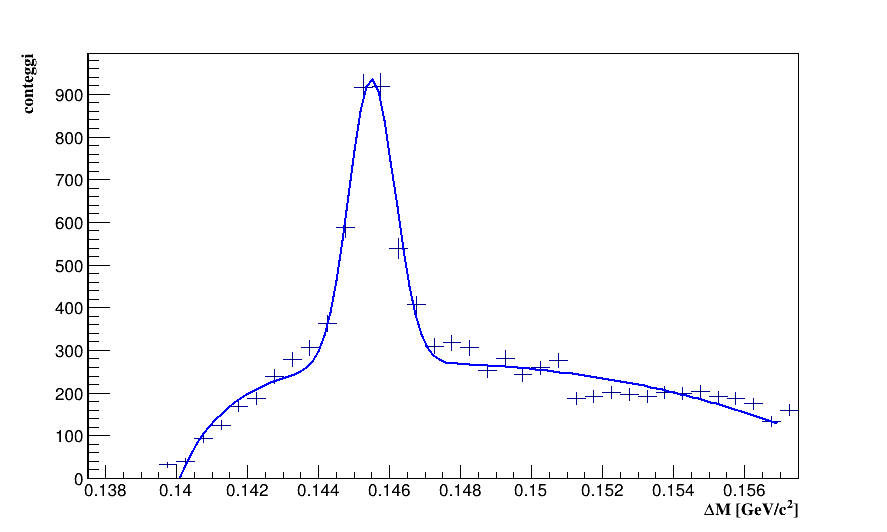
\includegraphics[width=0.48\textwidth]{AnalisiDati/pt_4_5_pol2.png}
        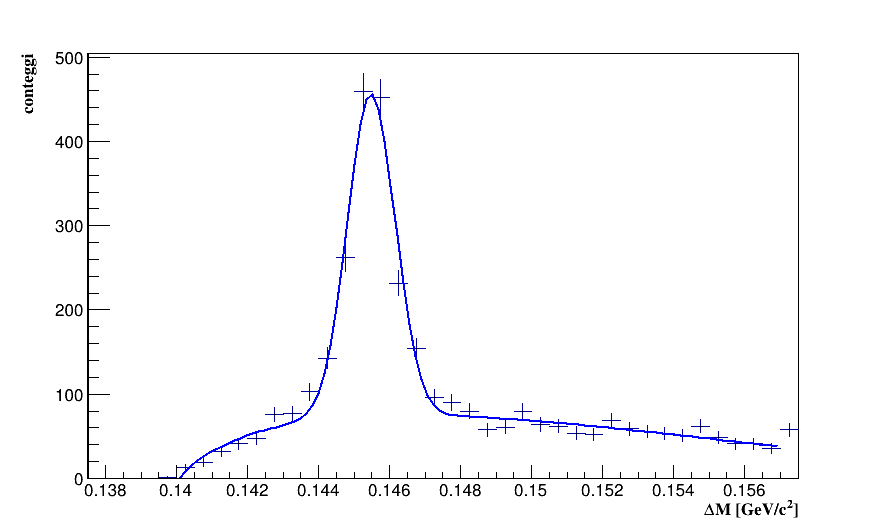
\includegraphics[width=0.48\textwidth]{AnalisiDati/pt_5_6_pol2.png}\\
        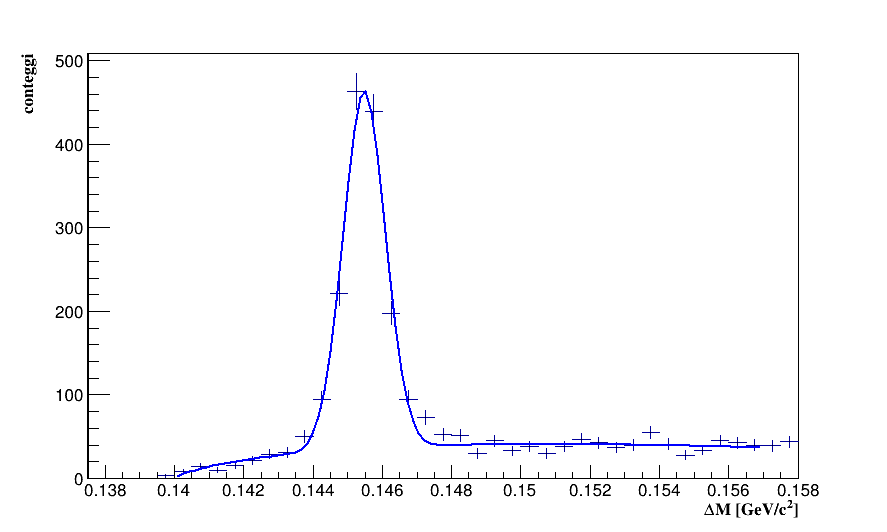
\includegraphics[width=0.48\textwidth]{AnalisiDati/pt_6_8_pol2.png}
        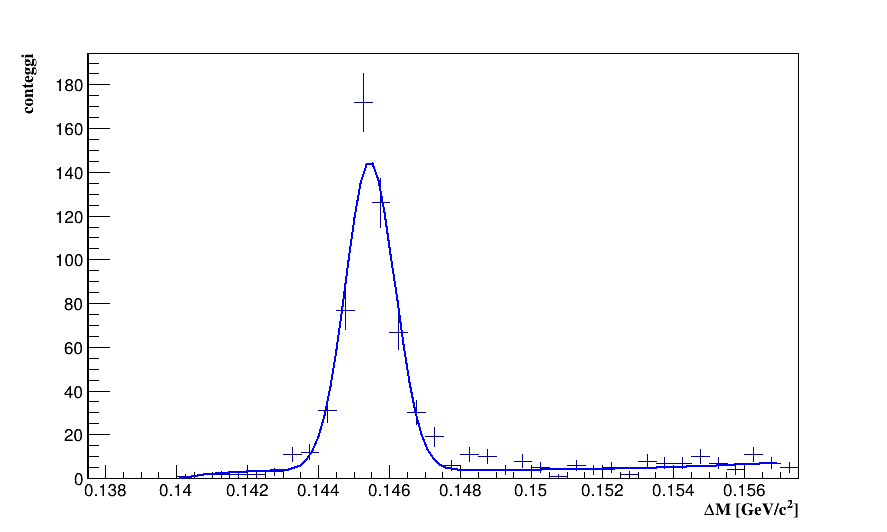
\includegraphics[width=0.48\textwidth]{AnalisiDati/pt_8_12_pol2.png}\\
       \caption{Distribuzione di massa invariante $\Delta M = M(\pi^+,\pi^+,K^-) - M(\pi^+,K^-)$, per gli intervalli di $p_T$ considerati nell'analisi e funzioni di fit $totale$ in blu.}
       \label{fig:fit}
   \end{figure}


\section{Risultati ottenuti}

Per determinare il numero di $D^{*+}$ ricostruite e selezionate con il metodo multivariato \`e stato calcolato l'integrale della funzione $totale$  in un intervallo definito come $\mu \pm 3 \sigma$ dove $\mu$  \`e il valore medio e $\sigma$ la deviazione standard della funzione Gaussiana. Il fondo residuo \`e stato stimato calcolando l'integrale della funzione $f$ nello stesso intervallo. Infine, per trovare la quantità di segnale, si è sottratto all'integrale della funzione $totale$ l'integrale del fondo. 
\\In figura \ref{fig:segnale} si riporta la quantità di segnale estratto dal fit delle distribuzioni di massa invariante in funzione del $p_T$ con l'errore statistico associato.

    \begin{figure}[htbp] 
        \centering
        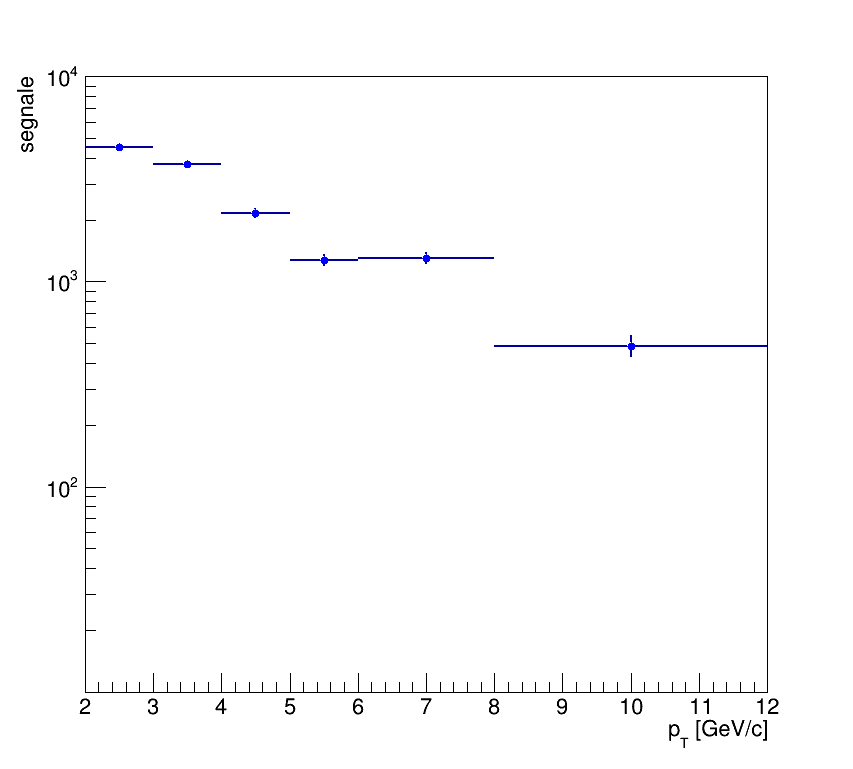
\includegraphics[width=0.8\linewidth]{AnalisiDati/segnale.png}
        \caption{Segnale estratto dal fit delle distribuzioni di massa invariante in funzione del $p_T$. La barra d'errore rappresenta l'errore statistico.}
        \label{fig:segnale}
    \end{figure}


In figura \ref{fig:fondo} è mostrata la quantità di fondo in funzione del $p_T$.

    \begin{figure}[h] 
        \centering
        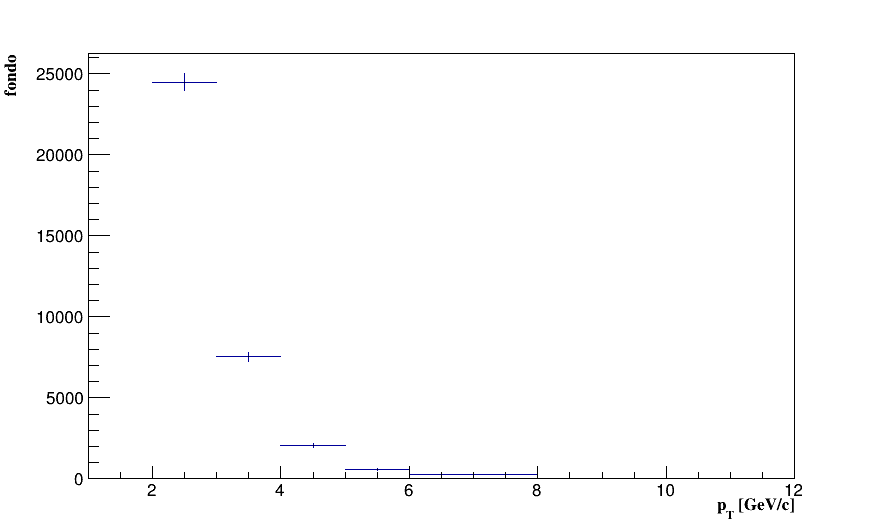
\includegraphics[width=0.8\linewidth]{AnalisiDati/fondo.png}
        \caption{Grafico della quantità di fondo in funzione del $p_T$, la barra d'errore rappresenta l'errore statistico.}
        \label{fig:fondo}
    \end{figure}
 
\clearpage
%\newpage
Si è calcolata anche la significanza, utilizzando la formula 
 
 \begin{equation}
     significanza = \frac{S}{\sqrt{S+F}}
 \end{equation}

dove $S$ è la quantità di segnale, mentre $F$ è la quantità di fondo. Anche in questo caso l'operazione è stata ripetuta per tutti gli intervalli di $p_T$ e con la propagazione degli errori si è ricavato l'errore statistico. Il grafico in figura \ref{fig:significatività} mostra il valore della significanza per gli intervalli di $p_T$ considerati. Si vede che si ha il massimo della significanza per l'intervallo di $p_T$ [3,4] GeV/c e il minimo per l'intervallo di $p_T$ [8,12] GeV/c.

    \begin{figure}[h] 
        \centering
        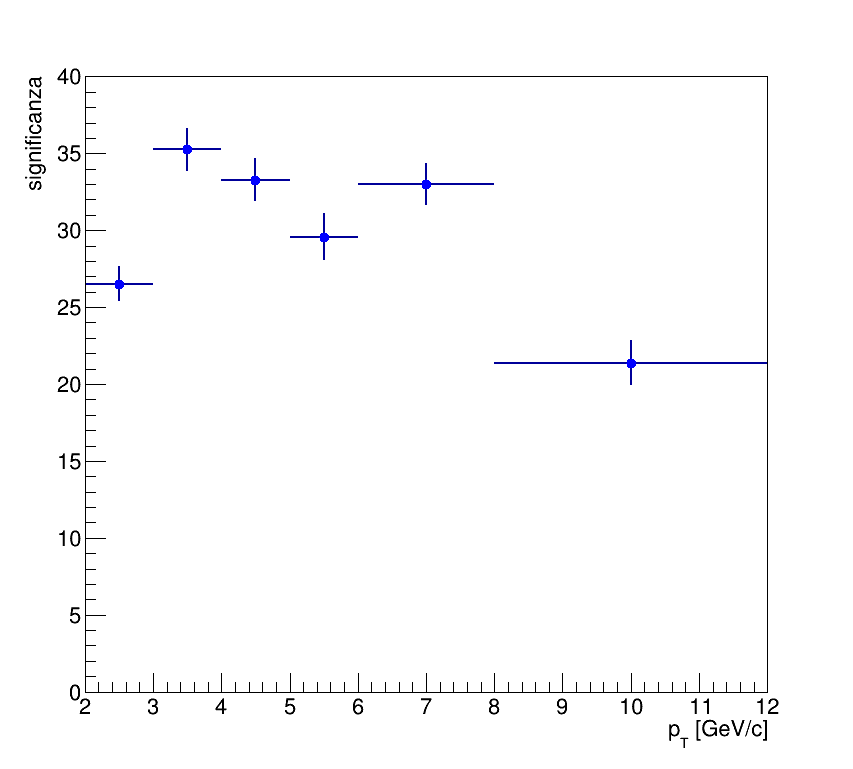
\includegraphics[width=0.8\linewidth]{AnalisiDati/significance_BDT.png}
        \caption{Significanza in funzione del $p_T$, la barra d'errore rappresenta l'errore statistico.}
        \label{fig:significatività}
    \end{figure}


La figura \ref{fig:s_b} riporta il grafico del rapporto tra segnale e fondo al variare del $p_T$. Si vede che il rapporto segnale su fondo aumenta al crescere del $p_T$, questo perché, come spiegato in precedenza, al crescere del $p_T$ il fondo combinatoriale diminuisce.

    \begin{figure}[htbp] 
        \centering
        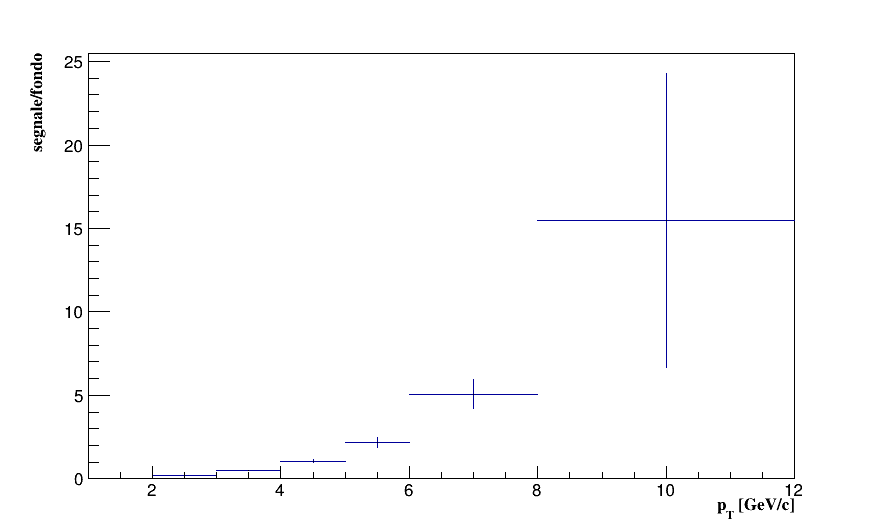
\includegraphics[width=0.8\linewidth]{AnalisiDati/s_b.png}
        \caption{Rapporto segnale su fondo in funzione del $p_T$, la barra d'errore rappresenta l'errore statistico.}
        \label{fig:s_b}
    \end{figure}
    
Infine, l'efficienza di selezione dell'algorimo \`e stata calcolata applicando l'algoritmo stesso ad un campione di solo segnale ottenuto da un Monte Carlo simile a quello usato per il training e calcolando il rapporto tra le candidate $D^{*+}$ selezionate come segnale dal BDT e la quantit\`a di segnale del campione.
In figura \ref{fig:efficienza_BDT} \`e mostrata l'efficienza dell'algoritmo utilizzato in questa tesi in funzione del $p_T$.
%come si calcola l'errore su un'efficienza?

\begin{figure}[htbp] 
        \centering
        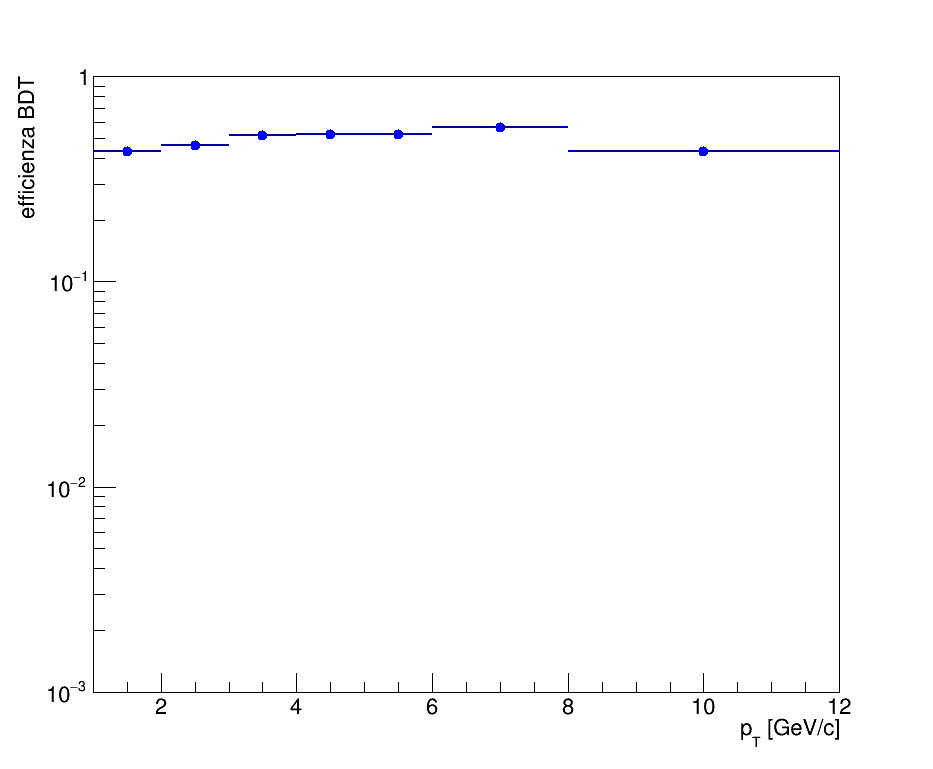
\includegraphics[width=0.8\linewidth]{AnalisiDati/eff_BDT.png}
        \caption{Efficienza dell'algoritmo di BDT in funzione del $p_T$.}
        \label{fig:efficienza_BDT}
    \end{figure}
    
\newpage
\subsection{Confronto con l'analisi standard di ALICE}    

I risultati ottenuti in questa tesi, selezionando le candidate $D^{*+}$ con un metodo di analisi multivariata sono stati confrontati con quelli ottenuti dall'analisi basata su selezioni topologiche\cite{dati_ALICE}.
In figura \ref{fig:confr_sign}, sono riportati i valori della significanza ottenuti con l'analisi eseguita con il BDT e quelli ottenuti con l'analisi standard di ALICE. Per gli intervalli di $p_T < 4$ GeV/c la significanza ottenuta con l'analisi eseguita con il BDT è più alta di quella ottenuta con l'analisi standard di ALICE di circa il $25\%$. Per l'intervallo di $p_T$ [4-5] le significanze ottenute con le due analisi sono compatibili, mentre per valori del  $p_T > 5$ GeV/c la significanza ottenuta dall'analisi standard di ALICE \`e maggiore di quella ottenuta con il BDT di pi\`u del $20\%$. 

    \begin{figure}[htbp] 
        \centering
        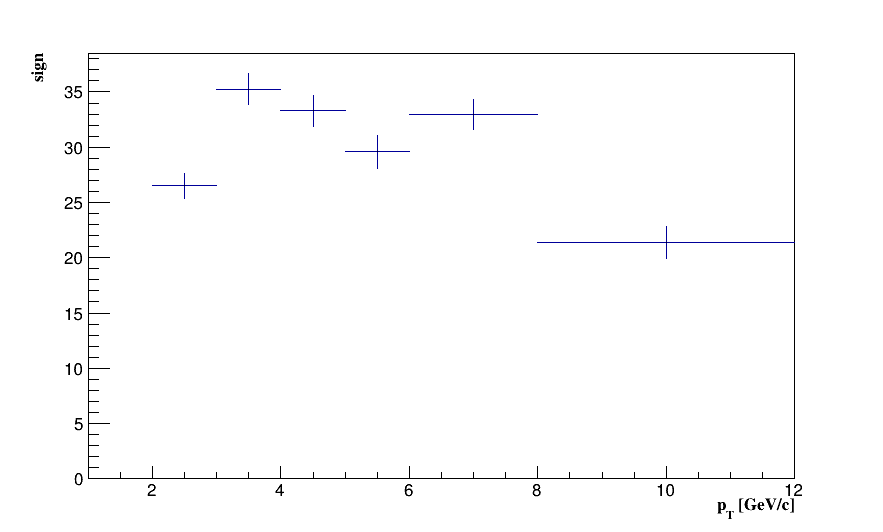
\includegraphics[width=0.8\linewidth]{AnalisiDati/significance.png}
        \caption{Significanza in funzione del $p_T$, in rosso per l'analisi standard di ALICE, in blu per l'analisi eseguita con il BDT presentata in questa tesi.}
        \label{fig:confr_sign}
    \end{figure}
  
L'efficienza del BDT \`e stata moltiplicata per l'accettanza geometrica del rivelatore così che potesse essere confrontata con quella dell'analisi standard di ALICE. %L'accettanza tiene conto sia della quantit\`a di particelle che possono essere rivelate dal rivelatore che delle pre-selezioni applicate sul campione di dati analizzato. 
In figura \ref{fig:eff_acc} \`e riportato il prodotto dell'efficienza del BDT per l'accettanza per i due metodi di analisi considerati. Dal grafico si vede che per valori di $p_T < 5$ GeV/c il valore dell'efficienza moltiplicato per l'accettanza del BDT \`e pi\`u alto di almeno l'$80\%$ rispetto a quello dell'analisi standard di ALICE, mentre per $p_T > 5$ GeV/c il valore dell'efficienza per l'accettanza dell'analisi standard di ALICE \`e maggior di quello del BDT al massimo del $30\%$.


    \begin{figure}[h] 
        \centering
        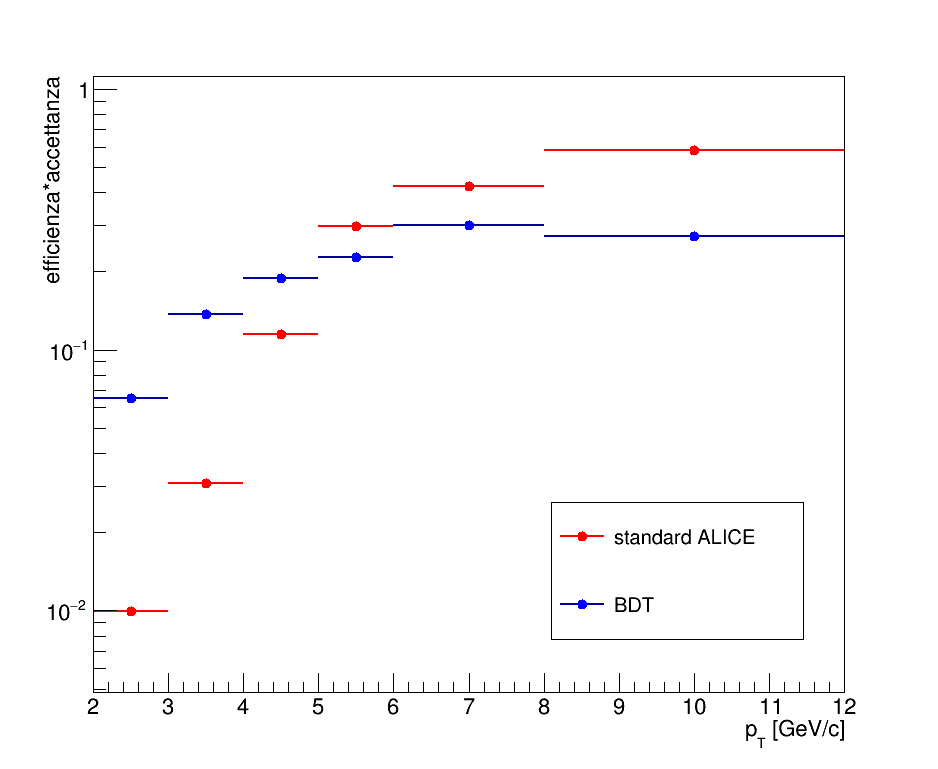
\includegraphics[width=0.8\linewidth]{AnalisiDati/eff_accett.png}
        \caption{Efficienza moltiplicata per l'accettanza in funzione del $p_T$, in blu per l'algoritmo del BDT e in rosso per l'analisi standard di ALICE.}
        \label{fig:eff_acc}
    \end{figure}

 
%sezione d'utro da modificare 


Infine è stata calcolata la sezione d'urto  della produzione del mesone $D^{*+}$  utilizzando la seguente formula:

    \begin{equation}
        \frac{d\sigma_{D^{*+}}}{dp_T} = \frac{1}{\Delta p_T} \frac{1}{BR} \frac{\frac{1}{2} N^{raw}(p_T) f_{prompt}(p_T)}{(\epsilon \times acc)(p_T) L_{int}}
    \end{equation}
    
dove $N^{raw}$ è il segnale della $D^{*+}$ estratto con il fit della distribuzione di massa invariante; $f_{prompt}$ è la frazione di $D^{*+}$ primarie prodotte nell'interazione protone-protone e non provenienti dal decadimento di altre particelle più pesanti, che sono dette secondarie (le candidate $D^{*+}$ selezionate contengono una misura delle due componenti); $\epsilon$ è l'efficienza dell'algoritmo (di cui \`e riportato il grafico in figura \ref{fig:efficienza_BDT}) moltiplicata per l'efficienza di ricostruzione; $acc$ è l'accettanza geometrica del rivelatore; $BR$ è il branching ratio del canale di decadimento considerato in questa tesi ($D^{*+} \rightarrow \pi^+ D^0(\rightarrow \pi^+ K^-)$) e vale $BR = 0.67 * 0.038 = 0.263 $. Il fattore $\frac{1}{2}$ tiene conto del fatto che vengono selezionate sia le particelle sia le antiparticelle, mentre si vuole considerare la sezione d'urto della sola particella.  
\\In figura \ref{fig:sezioneUrto} si mostra il grafico della sezione d'urto di produzione del mesone $D^{*+}$ in collisioni protone-protone ad un energia del centro di massa di 5 TeV ottenuto dall'analisi multivariata paragonato alla sezione d'urto ottenuta dall'analisi standard di ALICE. Le sezioni d'urto ottenute con i due metodi non sono compatibili considerando soltanto gli errori statistici e differiscono al massimo del 20\% con la differenza massima nell'intervallo []2,3] GeV/c. 
La differenza osservata potrebbe essere legata all'estrazione del segnale tramite la procedura di fit, ad una non completa rimozione del fondo nell'intervallo di $\Delta$M sotto il picco del segnale, oppure all'approssimazione nel calcolo della sezione d'urto in cui il termine $f_{prompt}$ \`e stato considerato uguale nei due casi. 

Se prendessimo in considerazione gli errori sistematici legati alla procedura di estrazione del segnale, al calcolo dell'efficienza di selezione del segnale e all'efficienza di tracciamento e di identificazione delle particelle, che non sono stati calcolati nell'ambito di questa tesi, le due sezioni d'urto risulterebbero compatibili entro gli errori sistematici \cite{dati_ALICE}).
 
 \begin{figure}[htbp] 
        \centering
        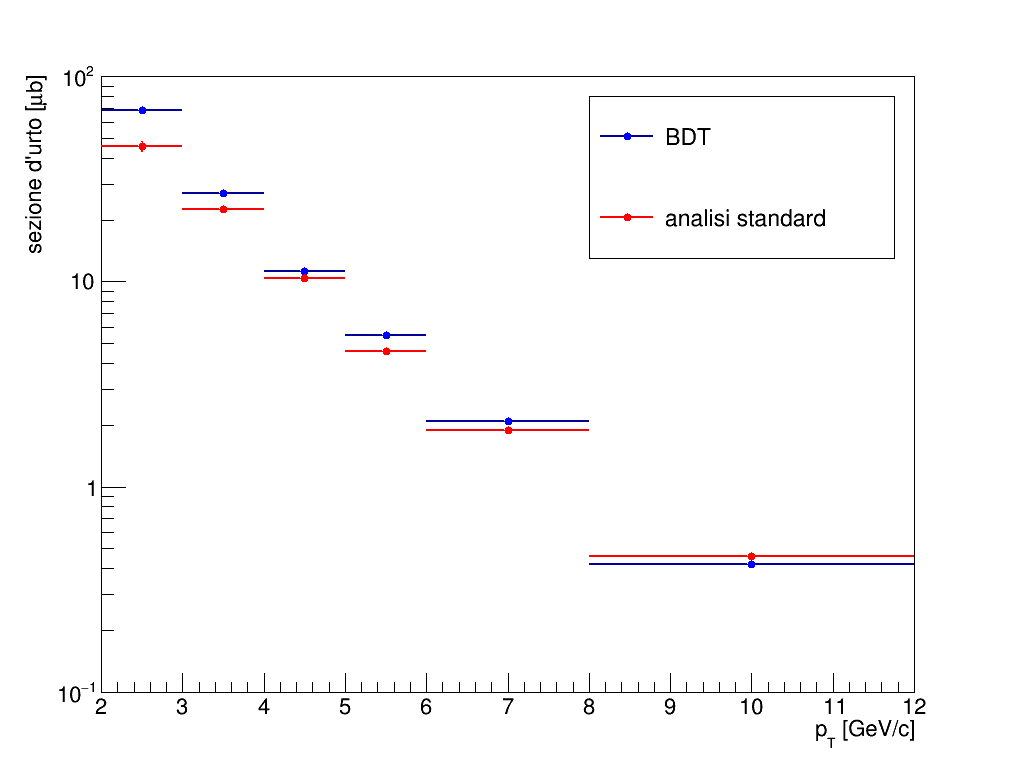
\includegraphics[width=0.8\linewidth]{AnalisiDati/sezioneUrto.png}
        \caption{Sezione d'urto del mesone $D^{*+}$ in funzione del $p_T$, in blu per l'analisi eseguita con il BDT e in rosso per l'analisi standard di ALICE.}
        \label{fig:sezioneUrto}
    \end{figure}
   
    
Per migliorare i risultati ottenuti con l'algoritmo di BDT per valori di $p_T > 5$ GeV/c, si potrebbe provare ad utilizzare un campione di dati pi\`u grande rispetto a quello utilizzato in questa tesi, cos\`i che l'algoritmo di BDT possa apprendere meglio nella fase di training come distinguere il segnale dal fondo. 
\\Inoltre per gli intervalli di $p_T > 5$ GeV/c si potrebbe provare ad utilizzare dei valori di taglio pi\`u bassi rispetto a quelli utilizzati in questa tesi cos\`i da preservare una maggiore quantit\`a di segnale.
    

